\documentclass[11pt, a4paper, twocolumn]{article}

\usepackage{config}
\usepackage{mathabx}
\usepackage{graphdefs}
\usepackage{pgfplots}
\pgfplotsset{compat=1.13}
\usepgfplotslibrary{statistics}
\newcommand{\norm}[1]{\left\lVert#1\right\rVert}
\bibliography{lit}

\begin{document}

\title{\texorpdfstring{\vspace{-0.5cm}}{}Algorithms for the Lower-Left Anchored Rectangle Problem}
\author{Anton Lorenzen}
\date{}

\maketitle

Allen Freedman \cite[p.~345]{tutte1969recent} posed the following combinatorial problem:
For some finite set of points in the unit square, we must find for each point $p$
a rectangle $R^p$ that has $p$ as its lower-left corner such that no two rectangles intersect.
If the origin is in the point set, can we cover at least half of the unit square in such rectangles?

Surprisingly little was known about the problem just a few years ago,
but it has received renewed attention in recent work.
Damerius et al. \cite{damerius2021greedily} show that the \textsc{TilePacking} heuristic
introduced below can always
cover 39\% of the unit square, but they also give an instance where this heuristic only
covers 43.3\%. No better ratio is known.

Rather than searching for the fastest algorithm attaining a known ratio, we therefore
consider the problem of maximising the area covered. Formally:

\begin{definition}[Lower-left Anchored Rectangle Packing]
    Given a finite set of points $P$ in the unit square $[0,1]^2$,
    find a rectangle $R^p = [p_x, r^p_x) \times [p_y, r^p_y) \subseteq [0,1]^2$ for each $p \in P$
    such that $R^p \cap R^q = \varnothing$ for all $p \neq q \in P$
    and the total area $\sum_{p\in P} \text{area}(R^p)$ is maximized (where $\text{area}(R^p) = (r^p_x - p_x)(r^p_y - p_y)$).
\end{definition}

Note that in particular $q \notin R^p$ for $p\neq q$.
Often, we will have that the origin $(0,0)$ is in $P$, but this is not required.
Indeed we will see, that the rectangle of the origin can always be chosen last, independent of
the other rectangles.

It is not known whether the problem can be solved in polynomial time,
but it is widely believed that this is not the case.
Antoniadis et al. \cite{antoniadis2019complexity} show that the related problem,
where the points $p$ need to be in the center of their rectangle $R^p$, is NP-hard.
However, their analysis does not translate easily to the present problem.

So how could one solve this problem? All the algorithms we discuss below
are based on a strategy Dumitrescu and Tóth \cite{dumitrescu2015packing} proposed.
They call a feasible solution \textit{pareto optimal} if no rectangle can be
made bigger without changing the others.
Then they describe how to choose for each pareto optimal solution a point $p$,
such that removing $R^p$ yields a pareto optimal solution for $P\setminus\{p\}$:

% Let us say that $q$ \textit{dominates} $p$ and write $p \leq q$, if $p_x \leq q_x$ and $p_y \leq q_y$.
Given a solution, we write $p \preceq' q$ if $[p_x, 1] \times [p_y, 1]$ intersects $R^q$.
In particular, if $R^q$ prevents the rectangle $R^p$ from growing, we will have $p \preceq' q$.
The transitive closure $\preceq$ of $\preceq'$ induces a partial order: This is clear except
in the antisymmetry case. But it can be seen by induction that if $p \preceq' q$ then
there is no $q'$ to the lower-left of $(\max \{p_x, q_x\}, \max \{p_y, q_y\})$ with $q \preceq q'$.

% Assume for the antisymmetry case that $p \neq q$, $p \preceq q$ and $q \preceq p$.
% Then we have some $p = s_1, \dots, s_n = q$ and $q = t_1, \dots, t_m = p$
% such that $s_1 \preceq' \dots \preceq' s_n$ and $t_1 \preceq' \dots \preceq' t_n$.

Therefore, we can pick any linear ordering compatible with the partial order $\preceq$ and
remove the smallest element $p$ (which prevents no rectangle from growing)
to obtain a pareto optimal solution for $P\setminus\{p\}$.
As the optimal solution is also pareto optimal, this implies that there is a
permutation $p_1, \dots, p_n$ of the points in $P$ such that we obtain the
optimal solution by choosing maximal rectangles for each $p_i$ in that order.
We call this permutation the \textit{optimal permutation}.
We do not have direct access to it, but we can simply try all possible
permutations and take the best result.

Unfortunately, this algorithm needs to consider $O(n!)$ permutations.
Harder \cite{harder2019anchoredrectanglecover} discovered that
the dynamic programming technique of the $O(2^n\,n^2)$ Held-Karp algorithm (for the
Traveling Salesman Problem)
also works for this problem. While we discuss that technique in section \ref{optimal},
packing according to special permutations has proven effective in practice.
Several variations are possible, which we discuss in section \ref{tiled} and section \ref{greedy}.
Finally, in section \ref{experiments} we show some charts that display the performance of the algorithms
on a dataset of random points.

\section{Tile Packing}
\label{tiled}

How could we place the rectangles in the optimal permutation? Dumitrescu and Tóth \cite{dumitrescu2015packing}
show that this can be done in time $O(n\log n)$ using the \textsc{TilePacking} algorithm:
To place $p_{i+1}$, we iteratively keep $R_i = \bigcup_{p=p_1}^{p_i} [p_x, 1] \times [p_y, 1]$.
We call $R_{i+1} \setminus R_i$ the \textit{tile} of $p_{i+1}$ and choose the best rectangle $R^{p_{i+1}}$ within
that tile. As every $R_i$ is a polygon consisting of at most $2(i + 1)$ points, we keep
all these corners (except $(1,1)$) in a binary search tree sorted by $x$-coordinate.
For point $p$ we then lookup the point $q$ in the binary search tree that is
closest to the right of $p_x$ and consider the points to the right of $q$
iteratively while their $y$-coordinate is bigger than $p_y$. From these points
$q = q^1, ..., q^m$, we choose the biggest rectangle $[p_x, q^i_x) \times [p_y, q^i_y)$
and delete them from the tree. Finally, we add $p$, $(p_x, q^1_y)$ and $(q^m_x, p_y)$ to the tree.
Clearly, this preserves the invariant that the tree contains the contour of $R_{i+1}$
and can be done in time $O(n \log n)$. It will also reach an optimal solution, as $p_i \precneq p_j$
for $i < j$ and therefore no $p_{i+1}$ has its optimal rectangle intersecting $R_i$.

\subsection{Permutations}

Note that \textsc{TilePacking} requires that the permutation obeys $\preceq$ if we seek an optimal solution.
However, we can run the algorithm on any permutation, as long as new points $p_{i+1}$ are
outside $R_i$. We say that $q$ \textit{dominates} $p$, written $p \leq q$ if
$p_x \leq q_x$ and $p_y \leq q_y$. Clearly, $p \leq q$ implies $p \preceq q$.
We call a set $P$ \textit{dominant} if for all $p \in P$ and $p \leq q$,
we have that $q \in P$. For the \textsc{TilePacking} algorithm to work we need that any
prefix $p_1, ..., p_i$ of the permutation is dominant. However, by the definition of $\preceq$ and
$\leq$, every prefix of the optimal permutation is dominant.

To obtain an approximate solution, we can choose to use any permutation obtained
by sorting the points according to a norm that guarantees that $\norm{p} < \norm{q}$ if $p < q$.
In the literature, the most commonly used norm is the 1-norm
(or Manhattan-norm) as this can also be seen as packing the points according to
their occurrence in a diagonal sweep from $(1,1)$ to $(0,0)$.
This is called the \textsc{TilePacking} \textit{heuristic}.

For random data, the $p$-norm with $p \approx 0.9$ performs best in practice.
Another interesting norm is the $-\infty$-`norm'
(computed by taking the minimum of the coordinates). The algorithm then
behaves as if we were growing the unit square towards the lower-left
and packing new points as they arrive (in a form of online strategy).

% \subsection{Simulated Annealing}

% If we seek an algorithm that performs better than \textsc{TilePacking} but does not have
% the runtime overhead of an optimal solution, we might try to improve an approximation iteratively.
% For example, we could take a norm-derived permutation and iteratively swap two points in the
% permutation if that improves our result. Unfortunately, there are some examples, where
% a non-optimal permutation can not be improved by swapping (only) two points. But if we
% are willing to sometimes swap also when we get no improvement (or even a loss), we
% can hope to achieve a good result. This is the idea behind simulated annealing.

% TODO, add example
% TODO, add exact algorithm

\section{Greedy Packing}
\label{greedy}

While the \textsc{TilePacking} algorithm is fast and easy to implement,
the result will not necessarily be pareto optimal if we do not use the optimal permutation.
In this section, we discuss the \textsc{GreedyPacking} algorithm which is very similar
to the \textsc{TilePacking} algorithm but always returns a pareto optimal solution.
Harder \cite{harder2019anchoredrectanglecover} showed how this can be achieved in
time $O(n^2\, \log n)$ and space $O(n^2)$.

However, we can improve this to $O(n^2)$ and $O(n)$ respectively if we perform the algorithm as follows:
In step 1, we find for the to-be-placed point $p$ the \textit{tile rectangle}: the smallest rectangle
that contains any rectangle $R^p$ that does not intersect any existing rectangle. In other terms,
we choose a point $q$ such that the rectangle $T$ spanned by $p$ and $q$ intersects only rectangles $R^s$
where $s$ lies in $T$ and $T$ is maximal. This can be done in time $O(n)$ by setting $q$ to $(1,1)$
and then inspecting all existing rectangles: if $R^s$ intersects $T$ and $s_x \leq p_x$,
we set $q_y = \min \{q_y, s_y\}$; if $R^s$ intersects $T$ and $s_y \leq p_y$ then we set $q_x = \min \{q_x, s_x\}$.

In step 2, we consider all points in $T$ to find the rectangle $R^p$. For this we maintain a list
of all points sorted by $x$-coordinate. We go through the list, and if a point $s$
lies in $T$, we set $R^p = \max \{R^p, [p_x, s_x) \times [p_y, q_y)\}$ and set $q_y = s_y$.

While \textsc{GreedyPacking} performs slightly better than \textsc{TilePacking}
in practice, there is no difference in the approximation guarantee
as Dumitrescu and Tóth \cite{dumitrescu2015packing} show. Indeed, if we place for
any point $(x,y)$ two new points directly below and to the left
at $(x - \epsilon, y)$ and $(x, y - \epsilon)$ and choose squares for them
greedily, directly after choosing a rectangle for $(x, y)$, their squares
will add at most $2\epsilon$ covered area and prevent any other uses of the tile of $(x, y)$.
As such, the result of Damerius et al. \cite{damerius2021greedily}, that \textsc{TilePacking} can not
cover more than 43.3\% for any instance, applies to \textsc{GreedyPacking} as well.

Unlike the \textsc{TilePacking} algorithm above, the \textsc{GreedyPacking} algorithm works even
for arbitrary permutations where a prefix of the permutation may not be dominant.
However, even with this new capability, the difference in runtime between the two algorithms seems big.
Next, we give a $O(n\log^2 n + k)$ algorithm that can perform both \textsc{TilePacking} and \textsc{GreedyPacking} on arbitrary permutations,
where $k$ is the sum of the number of points in all tile rectangles. For \textsc{TilePacking},
we have $k \in O(n)$, but for \textsc{GreedyPacking} $k \in O(n^2)$. Nonetheless,
in most instances we expect $k$ to grow smaller than $O(n^2)$ even for \textsc{GreedyPacking}.

We achieve this by implementing step 1 with a new datastructure that we call
a \textit{priority interval tree} and implementing step 2 with a range tree.
We give descriptions of some auxiliary datastructures below, which can also
be found in the computational geometry literature (see e.g. \cite[p.~135]{klein2006algorithmische})

\subsection{Finding all points in an interval}

Given a set of $n$ points $p$ on the line, we want to find for any interval
the set of points contained in that interval. We can construct a \textit{range tree}
for this in time $O(n \log n)$ that supports queries returning $k$ points in time $O(\log n + k)$.

We sort the points and create a balanced binary tree that has them as leaves.
In each internal node we store the smallest interval that contains all leaves
reachable from this node. Clearly, this can be done in time $O(n \log n)$.

For a query we then descend into the binary tree by going left if the interval
of the left internal node intersects the query interval and else right if the 
interval of the right internal node intersects the query interval
(if none of them intersects there are no points in the query interval).
This way we find the left-most point contained in the query interval in time $O(\log n)$.
Then we report all points to the right of the left-most point that are contained in the
query interval in time $O(k)$. This can for example be done by connecting all leaves in 
a linked list. Alternatively we can also walk through the tree in time $O(\log n + k)$.

\subsection{Finding all points in a rectangle}

Given a set of $n$ points $p$ in the plane, we want to find for any rectangle the set
of points contained in that rectangle. We can construct a \textit{2-dimensional range tree}
for this in time $O(n \log n)$ that supports queries returning $k$ points in time $O(\log^2 n + k)$.

First we take the set of $x$-coordinates of the points and construct a one-dimensional range tree
for them as above. For each leaf and internal node, we then construct another one-dimensional range tree
that contains all points with an $x$-coordinate in the interval associated to the node.

To do this efficiently, we first construct the $x$-coordinate range tree in time $O(n \log n)$ time as above.
Then we compute a list $L_2$ of all points sorted by $y$-coordinate and assign it to the root of the
$x$-coordinate range tree. Then we create such lists for the children of the root by sending a point in $L_2$ to the
left child if its $x$-coordinate is in the interval of the left child and sending it to the right child else.
We apply this step recursively and obtain at each node and leaf a list of all points in the associated $x$-interval. Clearly, every point
is only contained in $\lceil\log n\rceil$ many lists, so this can be done in time $O(n \log n)$.
Finally, we construct a range tree out of each list. Since the lists are already sorted, we can
construct a balanced binary tree for one in linear time. In total, this construction takes $O(n \log n)$ time.

For a given rectangle, we consider the maximal nodes in the $x$-coordinate tree whose associated
interval is completely contained in the $x$-interval of the rectangle. As there are only two of
them in any level of the tree, there are at most $O(\log n)$ in total which can be found in time $O(\log^2 n)$.
Then we start a $y$-interval lookup as above in each of the $x$-intervals. In total, a query thus
takes $O(\log^2 n + k)$ time.

\subsection{Finding all points in a half segment}

Given a set of $n$ points $p$ in the plane, we want to find for any half segment
($[x_1, x_2] \times [y_1, \infty)$), the set
of points contained in that half segment. We can construct a \textit{priority search tree}
for this in time $O(n \log n)$ that supports queries returning $k$ points in time $O(\log n + k)$.

First, we construct a range tree on the $x$-coordinates of the points (we keep duplicates
sorted by the respective $y$-coordinate). Then we sort the points by $y$-coordinates non-ascending
and insert them into the tree by placing them in the first empty internal node on the path
to their $x$-coordinate. This can be done in time $O(n \log n)$.

We can perform a query for a given half segment, similar to how we would look its
interval up in the range tree. However, we report the points along the way as we
find them and stop descending when the $y$-coordinate of the stored point becomes
too small.

\subsection{Finding all intervals containing a point}

Given a set of $n$ intervals in the line, we want to find for any point the
set of intervals that contain this point. We can construct an \textit{interval tree}
in time $O(n \log n)$ that supports queries returning $k$ intervals in time $O(\log^2 n + k)$.

First, we create two lists of the intervals sorted by the left and right endpoint respectively.
Then we create a balanced binary tree of the left endpoints where we store points in \textit{both}
the leaves and internal nodes. Recursively, we partition the intervals over the nodes of the tree.
We start by assigning all intervals to the root. Then we assign a interval to the left child if
it is completely to the left of the point at the current node, assign it to the right child if
it is completely to the right of the point at the current node and else keep it at the node.
In the end, we have at every node the intervals that contain the associated point of this node but no
point associated to a parent. At every node, we keep the intervals in two lists,
still sorted by left and right endpoint respectively. As any interval is contained in only one node,
this takes $O(n \log n)$ time.

For a given query point, we check if the query point is equal to the root and return the
list of intervals at the root in that case. Else we check if it is to the left or the right
of the root. If it is to the left, we return all intervals stored at the root that contain
this point (which we can find by binary search on the list sorted by left endpoints) and recurse
into the left subtree. Else, we perform binary search on the list sorted by right endpoints and
recurse into the right subtree. In total, we have $O(\log n)$ applications of binary search,
or $O(\log^2 n + k)$ time in total.

\subsection{Finding the $y$-smallest interval containing a point}

Below we are not interested in finding all intervals, but rather we want to
find the `smallest' one. To do this, we will need a datastructure
which we call a \textit{priority interval tree} as
we have not seen described before (although it likely exists already).

Given a finite set of $n$ $x$-axis-parallel line segments in the plane,
we want to find for any point $q$ the line that is hit first when
we shoot a $y$-axis parallel ray from $q$ to the top. In other words,
we look for the interval $I = [i_1, i_2] \times \{i_y\}$ such that $i_1 \leq q_x \leq i_2$, $i_y \geq q_y$
with $i_y$ smallest among such intervals. Our datastructure can be constructed in time $O(n \log^2 n)$
and supports queries in time $O(\log^2 n)$.

We construct an interval tree as above, but instead of two lists, we store
two priority search trees at each node, that contain the left/right endpoints
of the intervals. At each node we have to solve the following problem:

Assume that we are given $n$ points in the plane, each shooting an axis-parallel
ray to the right. For a query point $q$, we want to find out which ray we hit first,
if we shoot an axis-parallel ray out from the query point to the top.
In other words, we are looking for the point $p$ such that $p_x \leq q_x$, $p_y \geq q_y$
and $p_y$ is smallest among all such points (or the message that no such point exists).
This problem can be solved by a priority search tree, as we can simply
search for the half segment $(-\infty, q_x] \times [q_y, \infty)$ and take the top-most
node we encounter on the search path.

When constructing the priority search we also have to sort the points by $y$-coordinate.
As a result the total time to construct a priority interval tree is $O(n \log^2 n)$.
Otherwise the analysis remains the same. Later, in our algorithm, we will insert intervals
dynamically. It is possible to support this in time $O(\log n)$ with no impact on query
times \cite{widmayer1993algorithmen}, but one might chose instead to use a simpler approach based on binary structures
and occasional rebuilding (see e.g. \cite[p.~110]{klein2006algorithmische}).

\subsection{Faster Algorithm}

To implement \textsc{GreedyPacking}, we will re-implement steps one and two above
using the advanced datastructures we just presented. For step one, we keep two
priority interval trees: one for $x$-axis parallel lines and one for $y$-axis
parallel lines. Whenever we place a rectangle, we insert its left and bottom
border into the respective tree. When we want to find $q$, we can look up the
point $p$ in the trees and set $q_x$ to the $x$ returned by the $y$-axis parallel tree
and $q_y$ to the $y$ returned by the $x$-axis parallel tree (or $1$ if the lookup fails).
To implement step two, we simply keep a two-dimensional range tree and look up all
the points in the tile rectangles $T$ from step one.

We can use the same algorithm for the \textsc{TilePacking} problem if we store
the left and bottom border of the tile rectangle in the priority interval trees,
rather than the left and bottom border of the rectangle itself. This implies that
the tile rectangles never intersect each other and so the total cost of the range
tree lookups is $O(n\log n)$.

\section{The optimal algorithm}
\label{optimal}

We have seen above that any optimal solution can be given by greedily selecting
rectangles in a specific permutation. This immediately suggests an $O(n!\,n \log n)$
algorithm combining a search over all $O(n!)$ permutations with the $O(n \log n)$
\textsc{TilePacking} algorithm above. However, there is a much better algorithm.

\subsection{Dynamic Programming}

To achieve a $O(2^n\, n\log n)$ algorithm, Jonathan Harder \cite{harder2019anchoredrectanglecover}
proposed to adapt the Held-Karp algorithm that finds an optimal solution to the Traveling Salesman Problem
by dynamic programming. Instead of considering all permutations, we find the best permutation for
any of the $O(2^n)$ subsets of the points. Indeed, if $\{p_1, \dots, p_k\}$ is a prefix of the optimal permutation,
then it is also the optimal permutation for the instance consisting only of the points $p_1, \dots, p_k$ (excluding
the origin). Thus, we can find the optimal permutation for $\{p_1, \dots, p_k\}$ by taking the best
permutation arising from appending $p_i$ to the best permutation of $\{p_1, \dots, p_m\} \setminus \{p_i\}$
for some $p_i \in \{p_1, \dots, p_m\}$.

Unfortunately, this algorithm is quite slow in practice.
Next, we discuss some heuristics for speeding it up further.

\subsection{The Dominance Directed Acyclic Graph}

Recall that $q$ \textit{dominates} $p$, written $p \leq q$ if
$p_x \leq q_x$ and $p_y \leq q_y$. Clearly, $p \leq q$ implies $p \preceq q$.
A set $P$ is \textit{dominant} if for all $p \in P$ and $p \leq q$,
we have that $q \in P$.

We want to consider the graph $G$ on the points with an edge $(q, p)$ if $p \leq q$
and there is no point $s$ with $p \leq s \leq q$. For a dominant set, we call its
neighbors in this graph the \textit{frontier}. In particular, by the definition of $\preceq'$,
for the optimal permutation $[p_1, \dots, p_n]$, we will have that
any $\{p_1, \dots, p_i\}$ is dominant with $p_{i+1}$ in its frontier. As such, we
only have to consider dominant subsets in the dynamic programming algorithm.
As Jonathan Harder points out, for instances where $G$ consists of $c$ paths
the dynamic programming algorithm runs in time $O(n^c)$.

To construct this graph, we first build the graph $\overleftarrow{G}$ consisting of all points and an edge $(p, q)$
if $p \leq q$. Then we consider for every edge $(u, w)$, if there is a point $v$ and edges $(u, v)$ and $(v, w)$.
If so, we mark this edge for deletion (but do not delete it yet). Finally, we delete all marked edges
and invert the graph. For $n$ nodes and $m$ edges, this procedure runs in time $O(nm)$.
In theory, we can achieve a better bound:
we can find out if there is such a point $v$ in constant time if we know for any pair of
nodes whether they are connected by a length-2-path.
This can be computed by squaring the adjacency matrix, yielding an $O(n^{2.373})$ algorithm.

% Unfortunately, the number of edges of $G$ can be $O(n^2)$, as the instance where all points lie on
% one of two nested hyperbolas shows. This makes the graph too expensive to compute for the fast greedy algorithms,
% but the graph is quite useful for speeding up the optimal algorithm. In particular, the optimal permutation
% can be constructed by repeatedly choosing the next element from the frontier of the existing elements.

\subsection{Implied rectangles}

Assume that we have already placed the rectangles for $\{p_1, \dots, p_k\}$. It may now occur that
there is some point $p_i$ that has no other point in its tile. Since we use the \textsc{TilePacking}
algorithm to place the rectangles, we can not make the solution worse by simply placing this rectangle
directly. We say that this rectangle is \textit{implied} by the partial solution for $\{p_1, \dots, p_k\}$.
In particular, for $k = 0$ this argument implies that the roots of the dominance DAG can be
placed greedily before we even start the dynamic programming algorithm.

We have found this to be an extremely useful optimization in practice, as any placing of $c$ rectangles
implied by a partial solution avoids updating $2^{c-1}$ subsets.

\subsection{Dijkstra's Algorithm}

Often the dynamic programming approach will continue to update from subsets that have hopelessly
wasteful optimal permutations. We can avoid this by using Dijkstra's algorithm on the space of
subsets: We think of the subsets as nodes in a graph and any two nodes $S_1, S_2$ are connected
by an edge if there is a point $p$ such that $S_1 \cup \{p\} = S_2$. We define the cost of
this edge to be the size of the white space (not covered by a rectangle) in the tile of $p$ when we
place it after placing the points of $S_1$. The dynamic programming approach above corresponds to
a breadth-first search of this graph; but we can do better by using Dijkstra's algorithm instead.
This yields an optimal permutation as maximising the coverage is the clearly same as minimizing the white space.

In other hard combinatorial optimization problems, Dijkstra's algorithm can restrict the search space
significantly \cite{hougardy2015dijkstra}. In these cases, Dijkstra is usually sped up by 
changing the edge costs through a feasible potential that acts as a lower bound on future costs.
This approach is very similar to the $\text{A}^*$ algorithm.

However, we observed only modest improvements --- and due to the higher overhead, Dijkstra's algorithm
can even be slower! We believe that a central reason for this is the lack
of a good lower bound on the future edge costs. While Antoniadis et al. \cite{antoniadis2019complexity}
give an algorithm that computes an upper bound on the coverage (and thus a lower bound on the white space),
this algorithm is prohibitively slow. Instead we use a simple lower bound that simply measures for each
point the white space in its smallest possible tile. This can be computed in time $O(n \log^2 n)$, but can
only identify around a tenth of the final white space in random instances.

\section{Experimental evaluation}
\label{experiments}



\begin{figure}
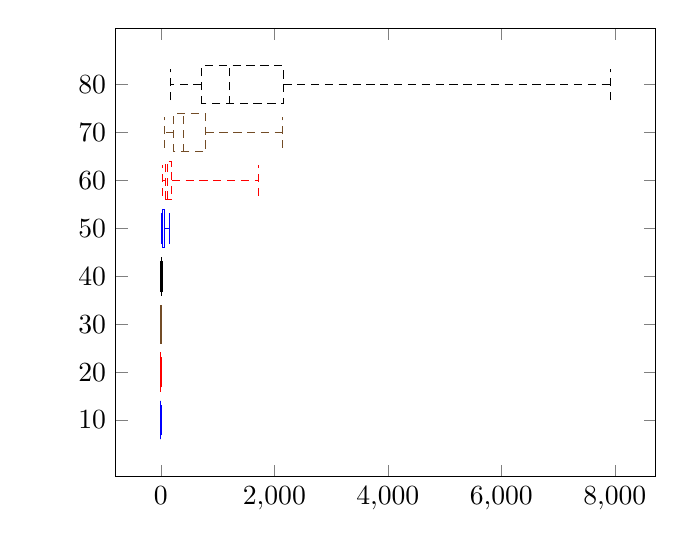
\begin{tikzpicture}
  \begin{axis}% [ boxplot/draw direction=y]
    [
    ytick={1,2,3,4,5,6,7,8},
    yticklabels={10,20,30,40,50,60,70,\phantom{100}80},
    % xtick={1,2,3},
    % xticklabels={Index 0, Index 1, Index 2},
    ]
    \addplot+[
    boxplot prepared={
      median=0,
      upper quartile=0,
      lower quartile=0,
      upper whisker=4,
      lower whisker=0
    },
    ] coordinates {};
    \addplot+[
    boxplot prepared={
      median=0,
      upper quartile=1,
      lower quartile=0,
      upper whisker=4,
      lower whisker=0
    },
    ] coordinates {};
    \addplot+[
    boxplot prepared={
      median=1,
      upper quartile=2,
      lower quartile=1,
      upper whisker=7,
      lower whisker=0
    },
    ] coordinates {};
    \addplot+[
    boxplot prepared={
      median=9,
      upper quartile=14,
      lower quartile=5.75,
      upper whisker=33,
      lower whisker=1
    },
    ] coordinates {};
    \addplot+[
    boxplot prepared={
      median=35.5,
      upper quartile=57,
      lower quartile=24.75,
      upper whisker=157,
      lower whisker=9
    },
    ] coordinates {};
    \addplot+[
    boxplot prepared={
      median=112.5,
      upper quartile=191,
      lower quartile=80.5,
      upper whisker=1720,
      lower whisker=27
    },
    ] coordinates {};
    \addplot+[
    boxplot prepared={
      median=402.5,
      upper quartile=788,
      lower quartile=231,
      upper whisker=2149,
      lower whisker=69
    },
    ] coordinates {};
    \addplot+[
    boxplot prepared={
      median=1208.5,
      upper quartile=2158.75,
      lower quartile=720.75,
      upper whisker=7925,
      lower whisker=171
    },
    ] coordinates {};
  \end{axis}
\end{tikzpicture}
\caption{Time (ms) for the Optimal Algorithm on $n$ uniformly distributed points; 100 instances}
\label{dynprogtime}
\end{figure}

We first evaluate the performance of the optimal algorithm.
Here we see the full effect of the optimizations described in that chapter:
The dynamic program on its own could only solve instances with 18 points in
a second, but with all optimization together, it is often possible to solve
even instances with 70 points! However, the optimizations of course do not
change the theoretical runtime of the algorithm and as such we can see
outliers that take much more time (see figure \ref{dynprogtime}).
Furthermore, the runtime still shows exponential characteristics and
so it seems infeasible to solve significantly larger instances.

\begin{figure}
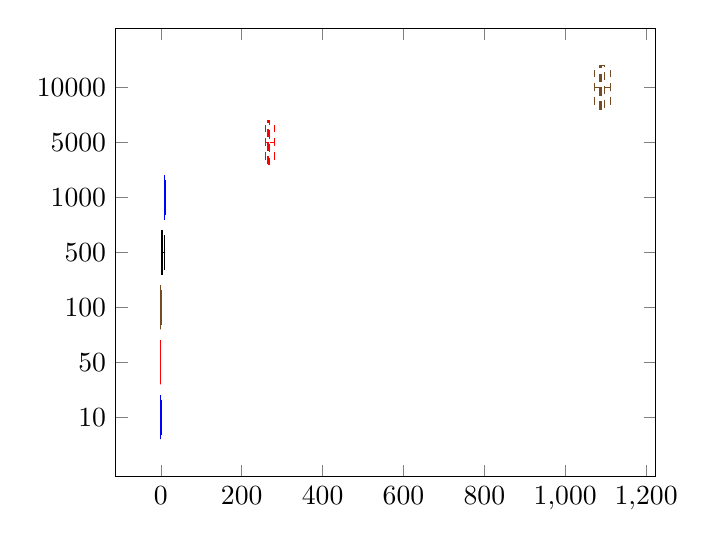
\begin{tikzpicture}
  \begin{axis}% [ boxplot/draw direction=y]
    [
    ytick={1,2,3,4,5,6,7},
    yticklabels={10,50,100,500,1000,5000,10000},
    % xtick={1,2,3},
    % xticklabels={Index 0, Index 1, Index 2},
    ]
    \addplot+[
    boxplot prepared={
      median=0,
      upper quartile=0,
      lower quartile=0,
      upper whisker=2,
      lower whisker=0
    },
    ] coordinates {};
    \addplot+[
    boxplot prepared={
      median=0,
      upper quartile=0,
      lower quartile=0,
      upper whisker=0,
      lower whisker=0
    },
    ] coordinates {};
    \addplot+[
    boxplot prepared={
      median=0,
      upper quartile=0,
      lower quartile=0,
      upper whisker=1,
      lower whisker=0
    },
    ] coordinates {};
    \addplot+[
    boxplot prepared={
      median=2,
      upper quartile=3,
      lower quartile=2,
      upper whisker=10,
      lower whisker=2
    },
    ] coordinates {};
    \addplot+[
    boxplot prepared={
      median=10,
      upper quartile=10,
      lower quartile=9,
      upper whisker=11,
      lower whisker=9
    },
    ] coordinates {};
    \addplot+[
    boxplot prepared={
      median=267,
      upper quartile=269,
      lower quartile=265,
      upper whisker=282,
      lower whisker=259
    },
    ] coordinates {};
    \addplot+[
    boxplot prepared={
      median=1088.5,
      upper quartile=1096,
      lower quartile=1083.75,
      upper whisker=1112,
      lower whisker=1073
    },
    ] coordinates {};
  \end{axis}
\end{tikzpicture}
\caption{Time (ms) for the Greedy Algorithm on $n$ uniformly distributed points; 100 instances}    
\label{greedytime}
\end{figure}

Naturally, the \textsc{TilePacking} and \textsc{GreedyPacking} algorithms run
much faster. We have found that even the quadratic greedy algorithm described at
the start of section \ref{greedy} can solve instances with ten thousand points
in about a second (see figure \ref{greedytime}). As such, we did not implement the more complicated algorithm
described in that section.

\printbibliography
\end{document}